\cleardoublepage



\chapter{Étude de fonctionnement}

La première partie de notre projet a consisté à étudier les différentes étapes du fonctionnement de notre solution : de la réception d'un SMS sur le smartphone à son affichage sur l'ordinateur, mais aussi de l'écriture d'un message sur l'ordinateur jusqu'à son envoi par le smartphone.
L'objectif de cette étude était de trouver la solution optimale que nous développeront pour ce projet.
Nous détaillerons plus précisément le choix du service proposé à l'utilisateur pour l'envoi du SMS depuis l'ordinateur.





%%%%%%%%%%%%%%%%%%%%%%%%%%%%%%%%%%%%%%%%%%%%%%%%%%%%%%%%%%%%%%%%%%%%%%%%%%%%%%%%%%%%%%%%%%%%%%%%%%%%
%%%%%%%%%%%%%%%%%%%%%%%%%%%%%%%%%%%%%%%%%%%%%%%%%%%%%%%%%%%%%%%%%%%%%%%%%%%%%%%%%%%%%%%%%%%%%%%%%%%%
%%%%%%%%%%%%%%%%%%%%%%%%%%%%%%%%%%%%%%%%%%%%%%%%%%%%%%%%%%%%%%%%%%%%%%%%%%%%%%%%%%%%%%%%%%%%%%%%%%%%
%%%%%%%%%%%%%%%%%%%%%%%%%%%%%%%%%%%%%%%%%%%%%%%%%%%%%%%%%%%%%%%%%%%%%%%%%%%%%%%%%%%%%%%%%%%%%%%%%%%%
%%%%%%%%%%%%%%%%%%%%%%%%%%%%%%%%%%%%%%%%%%%%%%%%%%%%%%%%%%%%%%%%%%%%%%%%%%%%%%%%%%%%%%%%%%%%%%%%%%%%

\section{Les application mobiles}

Il est nécessaire que l'utilisateur installe une application sur son smartphone pour réagir aux réception de SMS et aux demandes d'envoi de l'utilisateur.
\\


Lors de la réception d'un SMS, l'application va recevoir une événement puis va lire le dernier SMS reçu.
Une fois le contenu et l'expéditeur du SMS lus, l'application va envoyer le message "sur l'ordinateur" de l'utilisateur pour l'avertir de la réception.

Lors de la réception d'un message (contenu du SMS et destinataire) provenant de "l'ordinateur" de l'utilisateur, l'application va envoyer le SMS au destinataire.
Cet envoi doit bien évidemment se faire de manière automatique et transparente.

Le schéma \ref{schemaFonctionnement_applicationMobile} représente le fonctionnement global des applications mobiles qui seront utilisées dans notre projet.
\begin{figure}[!h]
	\center
	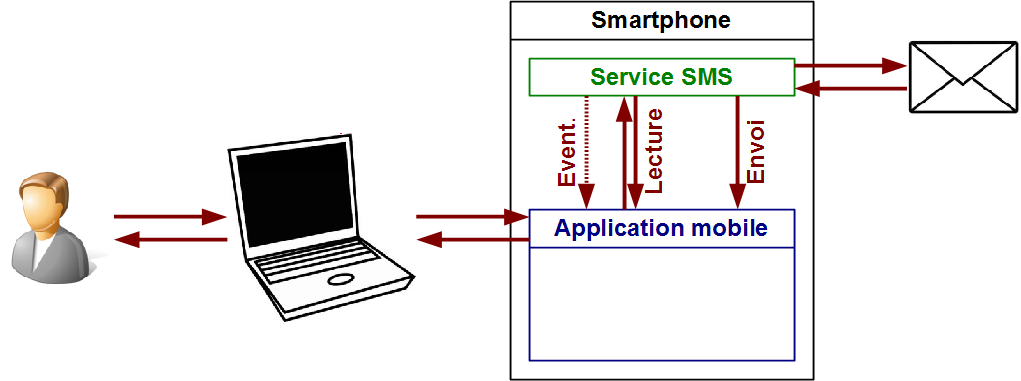
\includegraphics[width=0.9\textwidth]{img/schemaFonctionnement_applicationMobile.png}
	\caption{Applications mobiles : fonctionnement}
	\label{schemaFonctionnement_applicationMobile}
\end{figure}





%%%%%%%%%%%%%%%%%%%%%%%%%%%%%%%%%%%%%%%%%%%%%%%%%%%%%%%%%%%%%%%%%%%%%%%%%%%%%%%%%%%%%%%%%%%%%%%%%%%%
%%%%%%%%%%%%%%%%%%%%%%%%%%%%%%%%%%%%%%%%%%%%%%%%%%%%%%%%%%%%%%%%%%%%%%%%%%%%%%%%%%%%%%%%%%%%%%%%%%%%
%%%%%%%%%%%%%%%%%%%%%%%%%%%%%%%%%%%%%%%%%%%%%%%%%%%%%%%%%%%%%%%%%%%%%%%%%%%%%%%%%%%%%%%%%%%%%%%%%%%%
%%%%%%%%%%%%%%%%%%%%%%%%%%%%%%%%%%%%%%%%%%%%%%%%%%%%%%%%%%%%%%%%%%%%%%%%%%%%%%%%%%%%%%%%%%%%%%%%%%%%
%%%%%%%%%%%%%%%%%%%%%%%%%%%%%%%%%%%%%%%%%%%%%%%%%%%%%%%%%%%%%%%%%%%%%%%%%%%%%%%%%%%%%%%%%%%%%%%%%%%%

\section{Transfert du message}

%%%%%%%%%%%%%%%%%%%%%%%%%%%%%%%%%%%%%%%%%%%%%%%%%%%%%%%%%%%%%%%%%%%%%%%%%%%%%%%%%%%%%%%%%%%%%%%%%%%%
%%%%%%%%%%%%%%%%%%%%%%%%%%%%%%%%%%%%%%%%%%%%%%%%%%%%%%%%%%%%%%%%%%%%%%%%%%%%%%%%%%%%%%%%%%%%%%%%%%%%
%%%%%%%%%%%%%%%%%%%%%%%%%%%%%%%%%%%%%%%%%%%%%%%%%%%%%%%%%%%%%%%%%%%%%%%%%%%%%%%%%%%%%%%%%%%%%%%%%%%%

\subsection{Protocole XMPP}

%%%%%%%%%%%%%%%%%%%%%%%%%%%%%%%%%%%%%%%%%%%%%%%%%%%%%%%%%%%%%%%%%%%%%%%%%%%%%%%%%%%%%%%%%%%%%%%%%%%%

\subsubsection{Présentation}

\textit{Jabber}, maintenant appelé \textit{XMPP}\footnote{Site web : \href{http://xmpp.org/}{http://xmpp.org/}} (eXtensible Messaging and Presence Protocol) suite à sa standardisation, est un protocole de messagerie instantanée et de présence sur internet.
Bien que peu connu du public, ce protocole possède de très nombreux avantages :
\begin{itemize}
	\item standard ouvert : son fonctionnement est accessible par tous ;
	\item simple d'utilisation : les clients XMPP sont très simple d'utilisation car toute la complexité du protocole est situé coté serveur ;
	\item décentralisé ;
	\item confidentialité et sécurité ;
	\item ...
\\
\end{itemize}


Le protocole XMPP est de plus en plus utilisé par les services de messagerie instantanée, tels que iChat sur les produits Apple, le chat Facebook, ou Gtalk de Google que nous utiliserons dans ce projet.

%%%%%%%%%%%%%%%%%%%%%%%%%%%%%%%%%%%%%%%%%%%%%%%%%%%%%%%%%%%%%%%%%%%%%%%%%%%%%%%%%%%%%%%%%%%%%%%%%%%%

\subsubsection{Bibliothèques}

En raison de la nature dynamique, évolutive et ouverte du protocole XMPP, de très nombreuses bibliothèques sont disponibles (référencées sur le \href{http://xmpp.org/xmpp-software/libraries/}{site officiel} de la fondation) dans la majorité des langages de programmation.

Dans ce projet nous utiliserons \textit{aSmack}, un portage sous Androïd de la biblioyhèqhe Java \textit{Smack}, une bibliothèque Java, ainsi que \textit{XMPPFramework} une bibliothèque pour Objective-C.



%%%%%%%%%%%%%%%%%%%%%%%%%%%%%%%%%%%%%%%%%%%%%%%%%%%%%%%%%%%%%%%%%%%%%%%%%%%%%%%%%%%%%%%%%%%%%%%%%%%%
%%%%%%%%%%%%%%%%%%%%%%%%%%%%%%%%%%%%%%%%%%%%%%%%%%%%%%%%%%%%%%%%%%%%%%%%%%%%%%%%%%%%%%%%%%%%%%%%%%%%
%%%%%%%%%%%%%%%%%%%%%%%%%%%%%%%%%%%%%%%%%%%%%%%%%%%%%%%%%%%%%%%%%%%%%%%%%%%%%%%%%%%%%%%%%%%%%%%%%%%%

\subsection{Choix du protocole}

La première raison qui nous a poussé à choisir le protocole XMPP pour échanger les messages entre l'ordinateur et le smartphone est le fait qu'il s'agit du protocole de base de GTalk.
Initialement nous voulions envoyer et recevoir les messages depuis GTalk, comme nous l'expliquerons juste après dans la partie \ref{GTalk}.
Ce choix nous a donc paru judicieux car l'application mobile pourra échanger facilement des messages avec l'ordinateur sans aucun problème d'adaptation.

La seconde raison est le fait que la grande majorité des personnes possèdent un compte Google (Gmail), du fait de l'importance de Google sur l'univers d'Internet.
De plus les smartphones Androïd nécessitent l'association à un compte Google pour fonctionner (téléchargement d'application, mises à jour, ...), donc les utilisateurs n'auront pas à créer de compte Google ni même de compte XMPP.



%%%%%%%%%%%%%%%%%%%%%%%%%%%%%%%%%%%%%%%%%%%%%%%%%%%%%%%%%%%%%%%%%%%%%%%%%%%%%%%%%%%%%%%%%%%%%%%%%%%%
%%%%%%%%%%%%%%%%%%%%%%%%%%%%%%%%%%%%%%%%%%%%%%%%%%%%%%%%%%%%%%%%%%%%%%%%%%%%%%%%%%%%%%%%%%%%%%%%%%%%
%%%%%%%%%%%%%%%%%%%%%%%%%%%%%%%%%%%%%%%%%%%%%%%%%%%%%%%%%%%%%%%%%%%%%%%%%%%%%%%%%%%%%%%%%%%%%%%%%%%%

\subsection{Formatage}

Un SMS contient plusieurs informations : le numéro de téléphone de l'expéditeur ou du destinataire et son contenu.
Il va donc falloir définir un format à respecter dans lequel seront échangés les messages XMPP et qui va contenir l'ensemble de ces informations.
\\


Il existe plusieurs formats de données comme le XML (Extensible Markup Language), le JSON (JavaScript Object Notation) ou encore YAML (YAML Ain't Markup Language).
Nous avons décidé d'utiliser le \textit{JSON} du fait de sa popularité "à la mode", son aspect peux verbeux et sa bonne lisibilité.
\\


Voici l'exemple d'un message XMPP qui transitera du smartphone de l'utilisateur jusqu'à son ordinateur :
\begin{lstlisting}
{
    "action": "receive-sms-action",
    "authorPhoneNumber": "0123456789",
    "recipient": "987654321",
    "body": "Ceci est le contenu du SMS"
}
\end{lstlisting}
La première ligne corresponde au type de message : "receive-sms-action" lorsque l'utilise reçoit un SMS, "send-sms-action" lorsqu'il souhaite en envoyer un.
La seconde ligne correspond au numéro de l'auteur du SMS (facultatif lors d'un envoi).
La troisième ligne correspond au numéro du destinataire (facultatif lors de la réception).
Et enfin la dernière ligne correspond au contenu du SMS.



%%%%%%%%%%%%%%%%%%%%%%%%%%%%%%%%%%%%%%%%%%%%%%%%%%%%%%%%%%%%%%%%%%%%%%%%%%%%%%%%%%%%%%%%%%%%%%%%%%%%
%%%%%%%%%%%%%%%%%%%%%%%%%%%%%%%%%%%%%%%%%%%%%%%%%%%%%%%%%%%%%%%%%%%%%%%%%%%%%%%%%%%%%%%%%%%%%%%%%%%%
%%%%%%%%%%%%%%%%%%%%%%%%%%%%%%%%%%%%%%%%%%%%%%%%%%%%%%%%%%%%%%%%%%%%%%%%%%%%%%%%%%%%%%%%%%%%%%%%%%%%

\subsection{Fonctionnement}

Les messages sont échangés entre les deux clients XMPP : un présent dans l'application mobile et l'autre dans la solution présente sur l'ordinateur de l'utilisateur.

Le schéma \ref{schemaFonctionnement_protocoleTransfert} décrit les entités qui échangeront des messages en utilisant le protocole XMPP.
\begin{figure}[!h]
	\center
	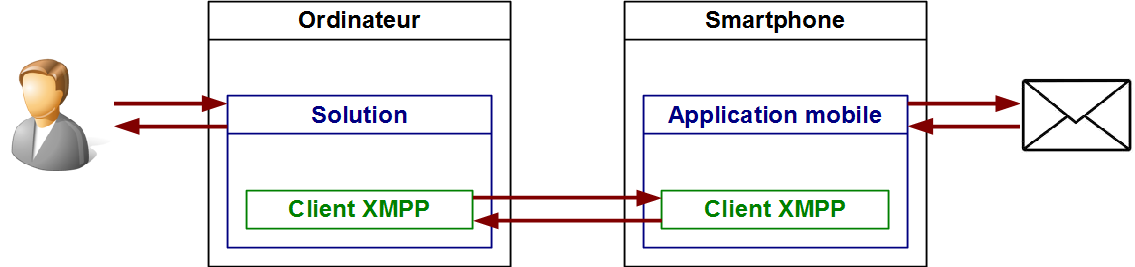
\includegraphics[width=0.9\textwidth]{img/schemaFonctionnement_protocoleTransfert.png}
	\caption{Transfert du message : fonctionnement}
	\label{schemaFonctionnement_protocoleTransfert}
\end{figure}





%%%%%%%%%%%%%%%%%%%%%%%%%%%%%%%%%%%%%%%%%%%%%%%%%%%%%%%%%%%%%%%%%%%%%%%%%%%%%%%%%%%%%%%%%%%%%%%%%%%%
%%%%%%%%%%%%%%%%%%%%%%%%%%%%%%%%%%%%%%%%%%%%%%%%%%%%%%%%%%%%%%%%%%%%%%%%%%%%%%%%%%%%%%%%%%%%%%%%%%%%
%%%%%%%%%%%%%%%%%%%%%%%%%%%%%%%%%%%%%%%%%%%%%%%%%%%%%%%%%%%%%%%%%%%%%%%%%%%%%%%%%%%%%%%%%%%%%%%%%%%%
%%%%%%%%%%%%%%%%%%%%%%%%%%%%%%%%%%%%%%%%%%%%%%%%%%%%%%%%%%%%%%%%%%%%%%%%%%%%%%%%%%%%%%%%%%%%%%%%%%%%
%%%%%%%%%%%%%%%%%%%%%%%%%%%%%%%%%%%%%%%%%%%%%%%%%%%%%%%%%%%%%%%%%%%%%%%%%%%%%%%%%%%%%%%%%%%%%%%%%%%%

\section{Service proposé à l'utilisateur}
\label{Service proposé à l'utilisateur}

%%%%%%%%%%%%%%%%%%%%%%%%%%%%%%%%%%%%%%%%%%%%%%%%%%%%%%%%%%%%%%%%%%%%%%%%%%%%%%%%%%%%%%%%%%%%%%%%%%%%
%%%%%%%%%%%%%%%%%%%%%%%%%%%%%%%%%%%%%%%%%%%%%%%%%%%%%%%%%%%%%%%%%%%%%%%%%%%%%%%%%%%%%%%%%%%%%%%%%%%%
%%%%%%%%%%%%%%%%%%%%%%%%%%%%%%%%%%%%%%%%%%%%%%%%%%%%%%%%%%%%%%%%%%%%%%%%%%%%%%%%%%%%%%%%%%%%%%%%%%%%

\subsection{GTalk}
\label{GTalk}

Google Talk, aussi appelé GTalk, est le client de messagerie instantanée proposé par Google.
Il est disponible à partir de la page web de Gmail, mais aussi en client Windows que l'on peut installer sur son ordinateur (Windows).

Initialement nous voulions utiliser ce client pour envoyer nos SMS pour la simple et bonne raison que de nombreux utilisateurs ont toujours le navigateur web ouvert, ainsi qu'un onglet avec leur boite mail.
De plus, nous voulions nous inspirer d'une solution existante qui utilise GTalk pour l'approfondir et lui ajouter de nouvelles fonctionnalités.

%%%%%%%%%%%%%%%%%%%%%%%%%%%%%%%%%%%%%%%%%%%%%%%%%%%%%%%%%%%%%%%%%%%%%%%%%%%%%%%%%%%%%%%%%%%%%%%%%%%%
%%%%%%%%%%%%%%%%%%%%%%%%%%%%%%%%%%%%%%%%%%%%%%%%%%%%%%%%%%%%%%%%%%%%%%%%%%%%%%%%%%%%%%%%%%%%%%%%%%%%
%%%%%%%%%%%%%%%%%%%%%%%%%%%%%%%%%%%%%%%%%%%%%%%%%%%%%%%%%%%%%%%%%%%%%%%%%%%%%%%%%%%%%%%%%%%%%%%%%%%%

\subsection{Problèmes}
\label{Problèmes}

%%%%%%%%%%%%%%%%%%%%%%%%%%%%%%%%%%%%%%%%%%%%%%%%%%%%%%%%%%%%%%%%%%%%%%%%%%%%%%%%%%%%%%%%%%%%%%%%%%%%

\subsubsection{Parler à soi-même}

Le protocole XMPP autorise et offre la possibilité de s'envoyer des messages instantanés à soi-même si l'expéditeur et le destinataire sont les mêmes comptes.

Cependant GTalk ne le permet pas, pour au moins deux raisons :
\begin{itemize}
	\item Pour envoyer un message à une personne il faut cliquer sur son lien dans la liste des contacts.
	Or notre propre adresse email n'y apparait pas même si l'on s'est ajouté dans nos contacts ;
	\item Gtalk n'affiche pas les messages que l'on s'envoie à soi-même, depuis un autre client XMPP comme une application mobile par exemple.
\end{itemize}

De ce fait il est donc nécessaire d'utiliser un compte intermédiaire.
On peut ainsi créer un compte spécial qui représenterai notre smartphone, et qui sera utilisé uniquement par l'application.
Le fonctionnement global de la solution se résumerait au schéma \ref{schemaFonctionnement_GTalk}.

\begin{figure}[!h]
	\center
	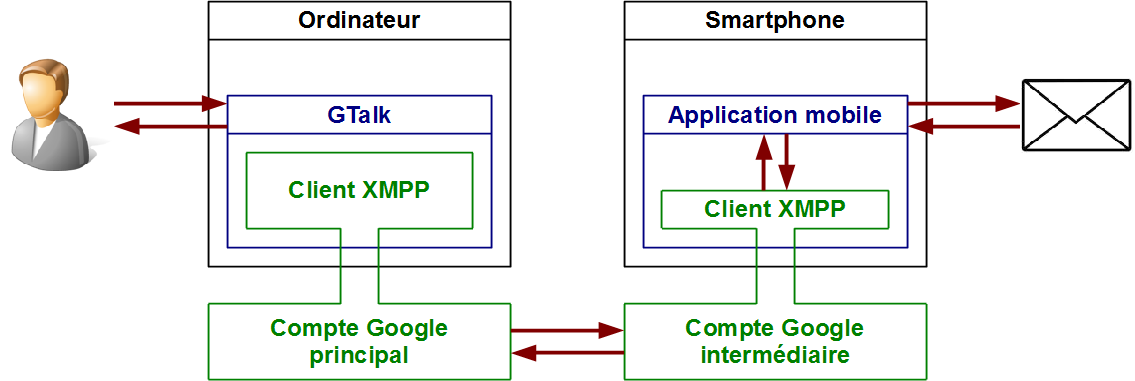
\includegraphics[width=0.9\textwidth]{img/schemaFonctionnement_GTalk.png}
	\caption{GTalk : Utilisation d'un compte intermédiaire}
	\label{schemaFonctionnement_GTalk}
\end{figure}

%%%%%%%%%%%%%%%%%%%%%%%%%%%%%%%%%%%%%%%%%%%%%%%%%%%%%%%%%%%%%%%%%%%%%%%%%%%%%%%%%%%%%%%%%%%%%%%%%%%%

\subsubsection{Praticité}

Pour différencier les SMS que l'utilisateur voudrait envoyer et les messages privés qui pourraient transiter par le biais du compte intermédiaire, nous voulions imposer une "règle", c'est à dire un format comme par exemple :
\begin{lstlisting}
sms 0123456789 Coucou, comment vas-tu ?
\end{lstlisting}

Mais cela impose à l'utilisateur de saisir un message correctement formaté.
De plus l'utilisateur doit saisir le numéro de téléphone du destinataire pour pouvoir envoyer le message, ce qui soulève les problèmes cités dans la partie \ref{Introduction de l'étude} du rapport.



%%%%%%%%%%%%%%%%%%%%%%%%%%%%%%%%%%%%%%%%%%%%%%%%%%%%%%%%%%%%%%%%%%%%%%%%%%%%%%%%%%%%%%%%%%%%%%%%%%%%
%%%%%%%%%%%%%%%%%%%%%%%%%%%%%%%%%%%%%%%%%%%%%%%%%%%%%%%%%%%%%%%%%%%%%%%%%%%%%%%%%%%%%%%%%%%%%%%%%%%%
%%%%%%%%%%%%%%%%%%%%%%%%%%%%%%%%%%%%%%%%%%%%%%%%%%%%%%%%%%%%%%%%%%%%%%%%%%%%%%%%%%%%%%%%%%%%%%%%%%%%

\subsection{Solution envisagée}

Suite aux inconvénients de GTalk mentionnés précédemment dans la partie \ref{Problèmes}, nous avons dû nous orienter vers une autre solution, indépendante de GTalk.
Plusieurs solutions sont possibles offrant chacune des avantages et des inconvénients.
\\


Le client lourd est un logiciel autonome que l'utilisateur doit "installer" sur son ordinateur.
Son fonctionnement est indépendant de tout serveur, hormis les échanges de données nécessaires aux traitements.
Pour notre projet, l'inconvénient de cette solution est l'obligation d'installation, ce qui peut poser problème lorsque l'on se trouve par exemple au travail ou que l'on utilise un ordinateur qui n'est pas le notre.
\\


Le site web est une application fourni par un serveur distant et accessible depuis n'importe quel navigateur internet.
Aucun programme ne devra être installé car cette solution est totalement indépendante de l'ordinateur de l'utilisateur.
Le seule pré-requis est un accès à internet, qui, quelque soit le type de solution proposé à l'utilisateur (client lourd, client léger, ...), est obligatoire pour l'utilisation du protocole XMPP.
C'est cette solution que nous utiliseront dans ce projet.
\\


Les différentes étapes du fonctionnement du site web est représenté sur le schéma \ref{schemaFonctionnement_siteWeb}
\begin{figure}[!h]
	\center
	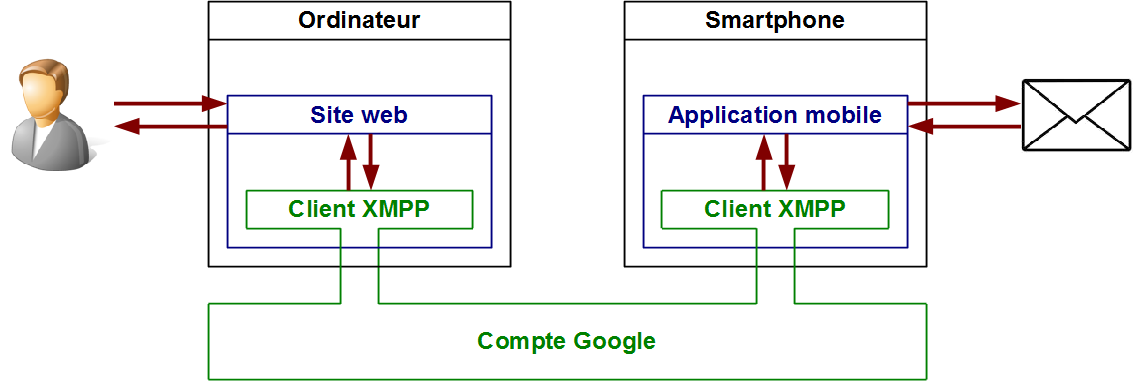
\includegraphics[width=0.9\textwidth]{img/schemaFonctionnement_siteWeb.png}
	\caption{Site web : Réception d'un SMS}
	\label{schemaFonctionnement_siteWeb}
\end{figure}
